\documentclass[conference]{IEEEtran}

\usepackage[dvips]{graphicx}
\usepackage{amsmath,amssymb}
\usepackage{algorithm}
\usepackage{algorithmic}
\usepackage{flushend}

\renewcommand{\sfdefault}{cmss}
\renewcommand{\rmdefault}{cmr}
\renewcommand{\ttdefault}{cmtt}

\usepackage{fontspec}
\setmainfont{FreeSerif}

\usepackage[font=small]{caption}
\captionsetup{singlelinecheck = false, justification=justified, labelsep=period}
\usepackage{float}
\usepackage[colorlinks,filecolor=blue,citecolor=green,unicode,xetex]{hyperref}
\usepackage{cmap}
\usepackage{amsmath,amssymb}
\usepackage[mathcal]{euscript}
\hypersetup{colorlinks=true, linkcolor=blue, citecolor=blue, filecolor=blue, urlcolor=blue, pdftitle=1, pdfauthor=, pdfsubject=, pdfkeywords=}

\sloppy
\clubpenalty=0
\widowpenalty=0
\raggedbottom

\begin{document}
\title{TRIK Studio: Technical Introduction}
\date{}%date stay empty

\author{
	\IEEEauthorblockN{Dmitry Mordvinov}
	\IEEEauthorblockA{
		St.-Petersburg State University \\
		St.Petersburg, Russia \\
		dmitry.mordvinov@se.math.spbu.ru
	}
\and
	\IEEEauthorblockN{Yurii Litvinov}
	\IEEEauthorblockA{
		St.-Petersburg State University \\
		St.Petersburg, Russia \\
		y.litvinov@spbu.ru
	}
\and
	\IEEEauthorblockN{Timofey Bryksin}
	\IEEEauthorblockA{
		St.-Petersburg State University \\
		St.Petersburg, Russia \\
		t.bryksin@spbu.ru
	}
}

\maketitle

\begin{abstract}
This paper presents TRIK Studio --- an environment for visual (and textual) programming of robotic kits, which is used in educational organizations across Russia and Europe. First part of the article provides overview of the system --- its purpose, features, differences from similar programming environments, general difficulties of robot programming and solutions proposed by TRIK Studio. Second part presents implementation details of TRIK Studio and its most interesting components. This article combines five fields of study: robotics, domain-specific visual modeling, education, formal methods and methods of program analysis. Main contribution of this article is detailed technical description of TRIK Studio as complex and successful open-source cross-platform robot programming environment written in C++/Qt, and first part of the article can also be interesting for teachers as it provides an overview of existing robot programming tools and related problems.
\end{abstract}

\section{Introduction}
\label{chapter:intro}
Current state of school education in computer science turned out quite like Seymour Papert predicted it to be. In 1967 he introduced a virtual Logo turtle, that is used to teach students programming at schools even nowadays. It is less known that Papert also used a mechanical robot turtle in his experiments, that was controlled from a computer~\cite{papert1980mindstorms}, and that made educational process much more entertaining. Today Papert's ideas are widely spread, a lot of schools are using robots to teach programming (for instance, in Russia robotics is a part of compulsory education program within the Technology course~\cite{luchin2016intro}). Several robotics educational kits are used, including Lego Mindstorms NXT, Lego Mindstorms EV3 (http://www.lego.com/en-us/mindstorms), TRIK (http://www.trikset.com/) etc.

The task of programming a robot is more complex than programming a virtual turtle: the program will be composed of motors power and sensor values manipulation instead of simple movements and turns. Therefore a lot of attention is paid towards robot programming environments. Many of them are based on visual, diagram languages since they are more intuitive and easy to learn than textual ones. Programming in such visual environments is performed by drag-and-dropping blocks using mouse and it makes programming available even to small kids, that cannot read yet. 

Popularity of visual languages in educational robotics is proven by a number of diagram-based programming environments in this field. The most known are Robolab~\cite{erwin2000lego}, NXT-G~\cite{kelly2010lego} and EV3-G~\cite{valk2014lego}, Scratch~\cite{resnick2009scratch} and Scratch-based environments (S4A (http://s4a.cat/), mBlock (http://www.mblock.cc/), Enchanting (http://enchanting.robotclub.ab.ca), ScrathDuino (http://www.scratchduino.ru/), Blockly (http://blockly.ru/) and App Inventor~\cite{wolber2011app}, 12Blocks (http://onerobot.org/products/12blocks/), Open Roberta~\cite{jost2014graphical}, Ardublock (http://blog.ardublock.com/), less known are Robo PRO~\cite{chang2006incorporating} for programming robots created with fischertechnik robotics kits or Program Maker for Scribbler robots and several tools for preschoolers: Lego WeDo Software~\cite{mayerova2012pilot}, Create~\cite{cross2013visual}, Wonder (https://www.makewonder.com/apps/wonder).

For the last decade educational robotics has been and still is a very promising scientific field, so in 2010s almost every major university in the world invested in development of projects in robotics. For example, in 2016 Harvard University presented the Root platform (http://http://wyss.harvard.edu/viewpage/629/), Carnegie Mellon University develops and promotes its Arts\&Bots project~\cite{cross2013visual}, MIT contributed delivering Scratch environment~\cite{resnick2009scratch} and so on. Detailed overview in Russian could be found in~\cite{mordvinov2016NONPUBLISHED}, and the authors conclude there that despite the variety of tools in this field there is no single one that can satisfy the needs of all educational organizations. Vast majority of such tools implement only the basic functionality (a visual editor for diagrams and an ability to run programs on robots autonomously or in a controlled manner from a computer), but they lack more advanced tools for teaching programming. Examples of such tools could be generation of readable textual code from created diagrams (that will help students to migrate from diagram-based to code-based programs), tools for debugging a program using virtual robot simulators or embedded tools for checking correctness of created programs (which could help teachers checking students' tasks). Some tools do have some of these advanced features, but often only some of them, and most of such programming environments are proprietary and pretty expensive for lots of schools.

Almost all aforementioned visual languages are based on control-flow computational model. Such a model is easier to comprehend, so it suits the purposes of education well. Nevertheless this model is not the best for programming robots since they are highly reactive by their nature: a program controlling a robot is basically a transformation of sensor signals into motor impulses. Reactive models are best expressed in data-flow languages~\cite{johnston2004advances}, where a program consists of a number of ``black boxes'', connected with data channels. Each such ``box'' (we will call it \emph{block}) has a fixed number of inputs and outputs, and its job is to transform input data into output data (we will call \emph{tokens} data transferring through channels). For instance, each robot's sensor is represented by a single block, that simply sends tokens with sensor data to its output. Many researchers note usability of visual data-flow languages comparing to a textual ones~\cite{johnston2004advances}, in particular because of clear visualization of data flows.

The idea of using data-flow programming languages in robotics is not a novel one, it was adopted in almost every toolset for programming industrial and laboratory automation systems, such as LabVIEW by National Instruments~\cite{kodosky1991visual}, Simulink~\cite{dabney2004mastering} and Microsoft Robotics Developer Studio~\cite{jackson2007microsoft}. They all have powerful backends (for example, Microsoft Robotics Developer Studio is being used on MySpace social network servers, see http://channel9.msdn.com/Shows/Communicating/CCR-at-MySpace for details) but are very complex and hard to learn. Thus they are used only in higher education~(\cite{stefanovic2011labview,yi2005labview}). School experiments with LabVIEW were popular in late 1990s~(\cite{cyr1997low,portsmore1999robolab}), which resulted in adaptations (like Robolab) replacing data-flow model  with control-flow model. So, there is a gap between simplified languages suitable for education and more elegant but complex industrial languages. There are attempts to adapt a data-flow model for educational robotics, for example a research group from New Zealand proposed the RuRu~\cite{diprose2011ruru} language. Nevertheless, to the best of our knowledge, there is still no production-ready data-flow-based programming environment suitable for secondary education today.

Current paper describes TRIK Studio programming environment, which attempts to solve the aforementioned problems. TRIK Studio is widely used in Russian education organizations (almost a hundred of schools and robotic clubs), several applications in Great Britain, France and Singapore are known. This paper presents technical overview of the programming environment; educational and methodical issues are not discussed in detail. Main scientific contribution of this article is a case study --- it describes an experience of creating robot programming environment specifically for school education and proposes ideas about language design and features which can be implemented in other such systems. It can also be viewed as an evidence of feasibility of using general-purpose domain-specific visual modeling platform to create domain-specific solution for wide audience.

\section{General description}
\label{chapter:generalDescription}

TRIK Studio is an environment that allows to program robots using diagram-based and textual languages. It emerged as a further evolution of QReal:Robots~\cite{terekhov2013robots} project, developed at Software Engineering chair of Saint-Petersburg State University. It supports Lego Mindstorms NXT, Lego Mindstorms EV3 and TRIK robotic kits. Each one of these kits can be programmed using one of two visual languages (more simple control-flow and more complex data-flow language) or one of a number of textual ones. For Lego NXT the programmer can choose between NXT OSEK C and Russian version of C (simplified for teaching textual programming), for TRIK --- JavaScript, F\#~\cite{kirsanov2014robotics} or PascalABC.NET~\cite{doliner2014basics}, for Lego EV3 the single official language for standard firmware, EV3 virtual machine's byte code, is supported.

A program created using one of visual languages (\textit{a visual program}) could be executed in one of three modes:
\begin{itemize}
    \item debugging using a virtual simulator,
    \item debugging on a PC while sending commands to a robot via USB, Bluetooth or Wi-Fi,
    \item textual code generation mode with subsequent upload and execution of the program on the robot.
\end{itemize}

In the first mode programs are being interpreted in a two-dimensional robot model (see Section~\ref{chapter:2dModel}). Users are able to create 2D model of the world surrounding the robot from walls and colored floor markup. According to TRIK Studio users this feature is very useful for initial program debugging, before any interaction with real robots. Our experience shows that this virtual model editor allows to recreate most of fields and obstacle courses used in competitions in robotics. Having such a simulation environment makes possible to learn robotics and programming even without having real robotic kits. There is also an experimental support for V-Rep 3D visual simulation environment~\cite{rohmer2013v}.

Debugging using a PC (so called \textit{interpretation mode}) is useful as a next step to see how the program behaves on a robot in real time. In this mode program variables' values can be observed in a special window (similar to how it is done in Watch list windows in almost all textual integrated development environments, IDEs) and sensor data can be displayed in a form of graphs. 

Code generation mode enables users to move from visual to textual programs. Generated code is displayed in an embedded QScintilla-based text editor, that provides a set of common features of a code editor: syntax highlighting, code autocompletion, undo/redo, brackets highlighting etc. TRIK Studio installation contains everything needed for building and uploading programs into a robot (a number of cross-compilers, WinSCP, Putty, etc.), and it makes compilation process and communication with robots transparent to its users.

TRIK Studio's user interface is shown on Fig.~\ref{image:TS_interface}. It displays a process of debugging a program that passes the maze using virtual simulation model.

\begin{figure*}[ht]
    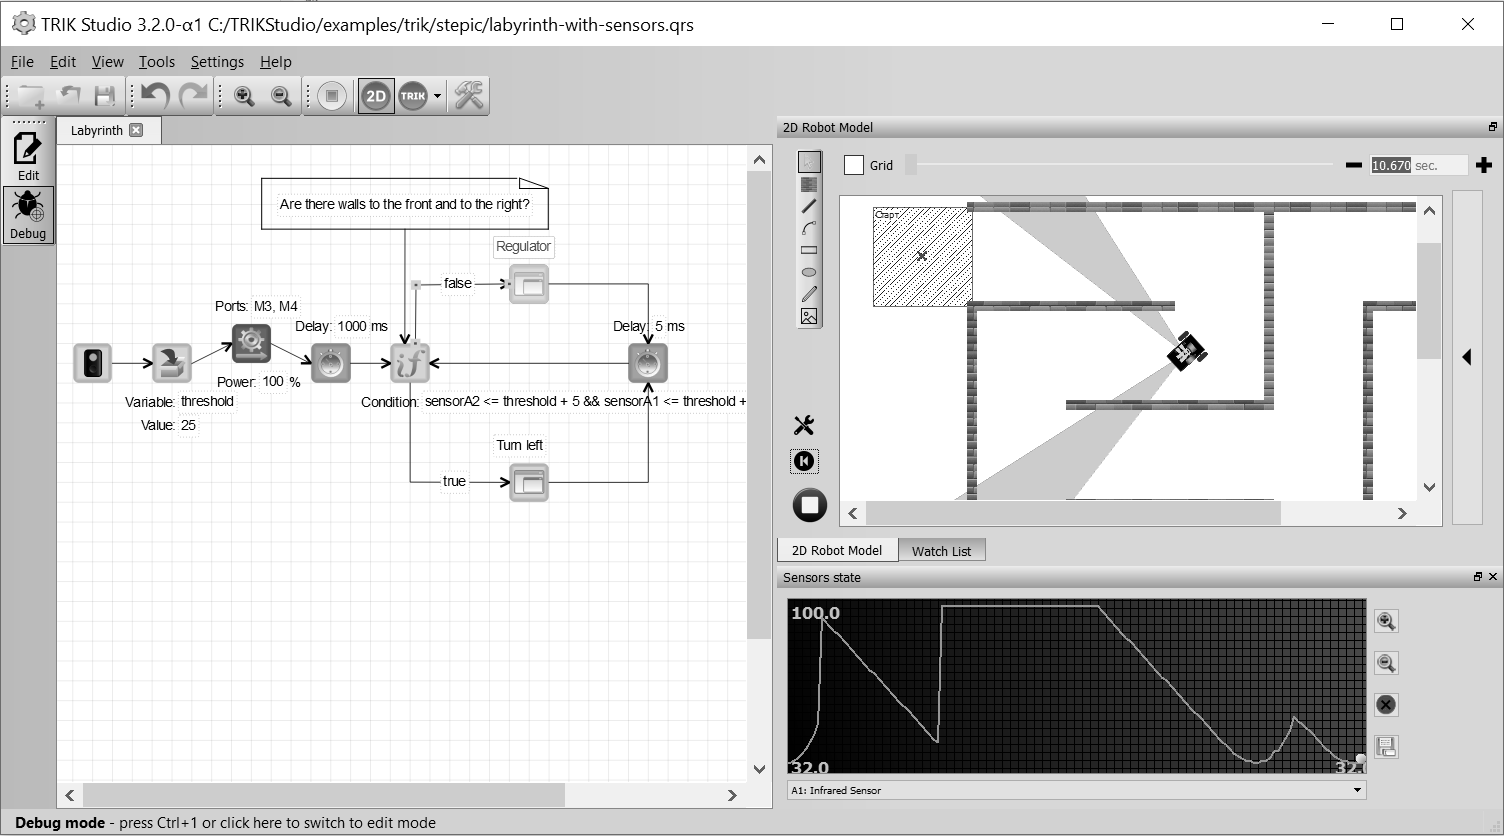
\includegraphics[width=\textwidth]{TS_CF_Labyrinth.png}
    \caption{TRIK Studio's user interface}
    \label{image:TS_interface}
\end{figure*}

In 2D simulation mode the automatic task checking feature is available (see Section~\ref{chapter:constraintsChecker}). Task checking program is written in internal event-based textual language, files containing virtual world model and task checking program can be distributed as tasks for students. Based on this feature a remote course has been launched on Stepik platform containing video lectures on cybernetics and robotics, numerous small tests and more than 20 tasks on educational robotics (see https://stepik.org/s/7qe3xj4Z). Each task can be downloaded, solved, checked within TRIK Studio on a student's computer, and uploaded to the server where the checking system will run it on its own tests (similar to ACM ICPC coding contests).

TRIK Studio is written in C++ using cross-platform Qt framework (https://www.qt.io/ru/), there are installers for Windows, Linux and Mac OS X operating systems. Because of the fact that official Lego NXT drivers are not available on Linux and Mac OS X x64, TRIK Studio contains our own implementation for them (see Section~\ref{chapter:communications} for details). The programming environment is completely free to use, open-source and is distributed under Apache License 2.0 license.

Aforementioned features distinguish TRIK Studio from all other similar tools. In fact among all mentioned in Section~\ref{chapter:intro} tools only 12Blocks have a comparable feature set, but it generates complex and unreadable code (for Lego NXT), does not have tools for checking tasks, is not free to use and does not have Russian support in it. Among the TRIK Studio drawbacks we should mention weak methodological support, limited only by embedded reference guide in Russian, a set of examples and the remote video course. Less important drawbacks will be mentioned in the following sections. 

The rest of the paper is structured as follows. Sections~\ref{chapter:controlFlowLanguage} and~\ref{chapter:dataFlowLanguage} briefly present TRIK Studio visual languages. Section~\ref{chapter:commonArchitecture} overviews the system architecture. Further sections describe separate TRIK Studio subsystems. Section~\ref{chapter:communications} presents robots communication infrastructure. Section~\ref{chapter:interpreters} describes visual language interpreters. The most interesting implementation details of code generators from control-flow language are provided in Section~\ref{chapter:generators}. Section~\ref{chapter:parser} presents textual languages parsing subsystem. Section~\ref{chapter:2dModel} presents implementation details of 2D simulation model subsystem. Section~\ref{chapter:constraintsChecker} describes task checking language and Section~\ref{chapter:conclusion} concludes the paper.

\section{Visual language for beginners}
\label{chapter:controlFlowLanguage}

The simplified control-flow based language (see Fig.~\ref{image:TS_CF_Example}) is the most often used one in TRIK Studio. It is a graph language, i.e. the program consists of nodes (\textit{blocks}) and edges (\textit{arrows}), organizing nodes into a directed control flow. To create a program users drag-and-drop necessary blocks onto the editor's scene, set their properties values and connect blocks with arrows. While being executed each block runs a sequence of basic commands and passes control to outgoing edges (to all or some of them depending on the block semantics). 

All language blocks are devided into four groups.

\begin{itemize}
    \item The first group is for blocks implementing basic algorithmic expressions, like a start and an end of a program or a subprogram, conditions, switches, arithmetic loops, blocks for parallel execution and for working with concurrent tasks (e.g. for merging and interrupting tasks), subprogram call block and a block for textual programming.
    \item The second group combines blocks working with robot peripherals. These are actions that don't require waiting. For example, there are blocks for setting motor powers, playing sounds, accessing robot video processing capabilities, synthesizing speach by given text, controlling motor encoders and LEDs, sending messages to other robots (a part of multi-agent interaction support), working with robot file system, etc.
    \item The third group consists of blocks, that ``freeze'' the control flow. They are a timer block waiting for a given number of milliseconds (similar to \texttt{msleep} function), blocks waiting for a given value from a given sensor or from an operator game pad, and a block waiting for receiving a message from another robot. 
    \item And finally, the fourth group contains blocks that provide drawing functions for basic primitives (the drawing is being performed on a robot's screen). Such primitives are lines, rectangles, ellipses, arcs, text and images. There are parameters to change color and width of pen and brush used in drawing. There are also special blocks that control robot model marker in a 2D simulation environment. It allows robot model to leave a trace on a ground while moving, similar to the Logo turtle.
\end{itemize}

\begin{figure*}[ht]
    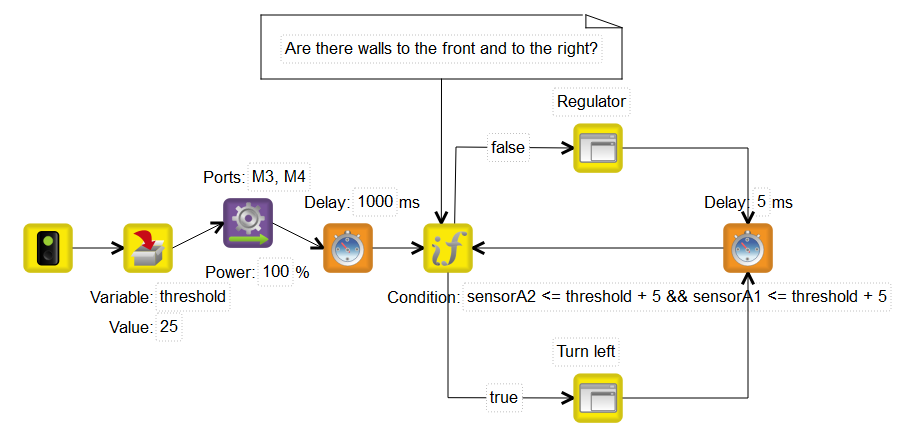
\includegraphics[width=0.8\textwidth]{TS_CF_Labyrinth_Diagram.png}
    \caption{The program of traversing the maze using right-hand rule. The first four blocks initialize the program: set the wall proximity variable, turn the robot motors on, after that the robot moves for one second to enter the maze. The second four blocks define the main control loop. Each ten milliseconds the robot checks using its infrared sensors if it can move forward or right (the \texttt{sensorA2 <= threshold \&\& sensorA1 <= threshold} condition). If it can move forward, the movement will be performed using proportional control over the right sensor data (the ``Regulator'' subprogram). If there are walls in front of the robot and to the right, it turn 90 degrees left (the ``Turn left'' subprogram).}
    \label{image:TS_CF_Example}
\end{figure*}

Properties of each block can be set both within the diagram editor's scene and using special property editor window. All block properties (where applicable) support computable expressions written in TRIK Studio embedded textual language -- a statically typed Lua dialect. The parsing module for this language is written using a parser combinator library in C++11, also created within TRIK Studio project. Type inference of the resulting abstract syntax tree is performed using slightly simplified Hindley-Milner algorithm~\cite{damas1982principal}.

The domain-specific approach (\textit{DSM-approach})~\cite{koznov2008} was employed to create the described visual language. The editor was created using QReal DSM platform~\cite{qrealMeta,kuzenkova2013qreal}. Language metamodel was defined using QReal's metaeditor, and a module implementing the editor was automatically generated using QReal's tools (as some other technologies like~\cite{bryksin2011ubiq}). Plugging this module into the QReal's platform core a complete visual IDE based on the given language is obtained. This IDE ``inherits'' all tools and features of the DSM platform, including modern user interface, mouse gestures recognition support for creating diagram elements~(\cite{osechkina2010gestures,osechkina2012multistroke}), copy-paste and undo/redo frameworks, zooming tools, tools for creating several types of edges on diagrams, model explorers, touch screens support and many more. According to its users TRIK Studio's user interface is much more usable and ergonomic than in any other such programming environment, and we spent only about three man-days working on it. We believe that it acknowledges the choice of QReal DSM platform as an underlying technology, but we have to note that while creating tool support for TRIK Studio numerous improvements were made to the QReal platform itself.

\section{Visual language for advanced users}
\label{chapter:dataFlowLanguage}

Users that mastered the control-flow language can move on to a more complex, but more convenient and powerful data-flow visual language. Unlike control-flow programs where control is passed according to edges between nodes, in data-flow programs blocks are executed simultaneously and communicate with each other by sending data tokens via channels. For instance, a data-flow program can have several entry points (most often they are robot sensors that send each other data for processing in chains), while a control-flow program must always have a single entry point. This language also has blocks for basic algorithmic expressions, blocks for interaction with all robot devices, drawing blocks, etc. Almost always data-flow programs turn out to be more concise than their control-flow analogues. For example, Fig.~\ref{image:alongTheBox_CF_DF} shows a proportional controller implemented in the control-flow language is compared with proportional-derivative controller implemented in the data-flow language.

\begin{figure}[ht]
    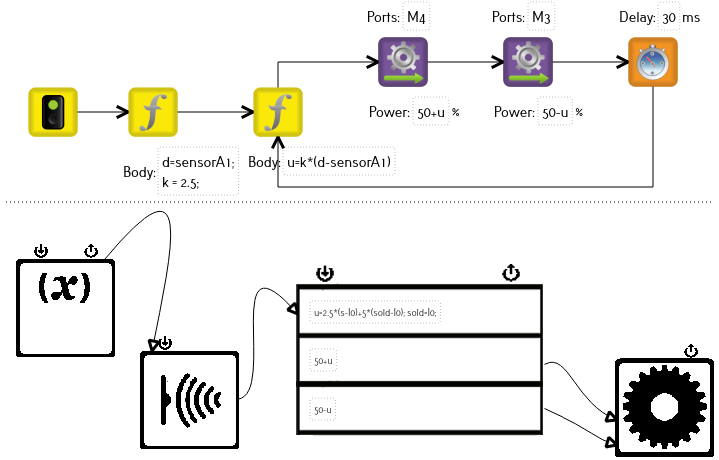
\includegraphics[width=\columnwidth]{TS_AlongTheBox_Comparison.png}
    \caption{Controllers implemented in different visual languages}
    \label{image:alongTheBox_CF_DF}
\end{figure}

To make transition to this ``advanced'' language simpler it maintains some kind of conceptual compatibility with the control-flow language. Blocks can also be organized in a chain with explicit passing of control, to make it possible most blocks have a special activation port that ignores all input data and just executes the block like it was in the control-flow case. So users can write programs like they used to and move on to using smaller number of blocks as they gain more experienced.

Expressive power of the language allows to use it for creating well-known complex robot control systems like Rodney Brooks's categorical architecture~\cite{brooks1986robust}, Johnathan Connell's ``colony'' architecture~\cite{connell1989colony}, Ronald Arkin's behavioral navigation~\cite{arkin1987motor}, or DAMN distributed navigation approach~\cite{rosenblatt1997damn}. Proof of this statement worth a separate paper and is not provided here. Another ideas on this matter could be found, for example, in~\cite{simpson2009toward} or~\cite{banyasad2000visual}.

It worth noting that in the time of writing TRIK Studio has only experimental support for data-flow language and it is not included in the officially distributed package. The source code of the editor and all appropriate tool support is freely available and could be compiled with the TRIK Studio's source code (for the source code see https://github.com/ZiminGrigory/qreal/tree/DFVPL).

\section{General architecture}
\label{chapter:commonArchitecture}

This section aims to structure the information given previously describing TRIK Studio's architecture: most of the features described here were already mentioned above. All diagrams presented here are distilled of numerous architectural and implementation details that though could be interesting in a context of such a paper, still left aside limited by the paper size.

Fig.~\ref{image:commonTSArch} presents high-level architecture of TRIK Studio. The system has a number of layers, each one implementing specific set of functionality and having strictly defined API. The lowest layer is libraries implementing interaction with real robots and virtual robot models. They are used to implement a hierarchy of robot devices (sensors, motors, displays, speakers, game pads, control buttons, etc.), which in their turn are used to specify high-level robot models for different robotic kits. Such robot model specifications are grouped into modules that are plugged into TRIK Studio's core, where they are used by other subsystems (e.g. interpreters and code generators that are structured as plug-in modules too).

TRIK Studio core in its turn is a plug-in module for QReal DSM platform. It modifies QReal's user interface, adding several toolbars and windows, like 2D simulation window, sensor configuration window, variable watch list and graphs window, etc. The core loads all robot model specifications and provides them to all other subsystems, provides user with information about interpretation and code generation processes, etc. Along with modules implementing TRIK Studio tools, visual language modules (that are created using the QReal platform itself) are also plugged into the QReal core. Implementation details of lower layers from Fig.~\ref{image:commonTSArch} are provided in the subsequent sections.

\begin{figure*}[ht]
    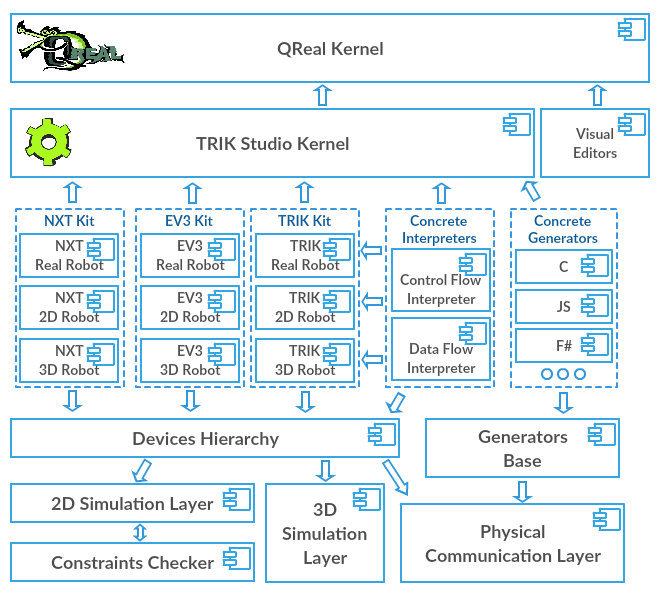
\includegraphics[width=0.6\textwidth]{TS_Common_Architecture.png}
    \caption{High-level TRIK Studio architecture}
    \label{image:commonTSArch}
\end{figure*}

Making the architecture highly modular allowed to provide flexible customization of the installation process: users can explicitly select which components they are interested in and install only them (for example, if someone has only a Lego EV3 kit, he or she does not need support for Lego NXT and TRIK robots, and the target installation will not contain such files). Furthermore, such an approach is highly compatible with packet-based software install systems in Linux. The architecture also benefits from such separation since the components become very low coupled: TRIK Studio's core, for example, is very minimalistic, it does not ``know'' about all features that the IDE provides and contains only objects and interfaces common to all robotic kits and models. API of each layer is fixed and well-documented, so it allows independent community developers to create extension modules supporting new languages, robotic kits and tools.

\section{Communications with robot controllers}
\label{chapter:communications}

This section discusses the subsystem handling TRIK Studio interaction with robots over different protocols. It is one of the lowest abstraction layers shown in Fig.~\ref{image:commonTSArch}. Its API provides the following operations: 

\begin{itemize}
    \item changing current transmission medium (currently Bluetooth, Wi-Fi and USB are supported),
    \item setting device address in terms of a chosen medium (e.g. COM port number in case of Bluetooth, IP address or host name in case of Wi-Fi),
    \item connecting to and disconnect from a remote device,
    \item transferring byte arrays to a remove device,
    \item handling receiving data from a remove device,
    \item handling connection status change (i.e. connection setup or termination events),
    \item handling errors.
\end{itemize}

USB communication is implemented using \texttt{libusb} library (http://libusb.org/), Bluetooth communication is based on \texttt{QextSerialPort} library (https://github.com/qextserialport/), Wi-Fi communication is implemented over TCP and UDP protocols using \texttt{QtNetwork} library, complex communication protocols (like configuration of TRIK robots before running programs) are built upon \texttt{Qt State Machine Framework}. The communication process is run in a separate thread to prevent freezing the main user interface. Particular implementations of communication mechanisms could be extended and replaced with other components. For examples, it is done for integrating TRIK Studio with the official Lego NXT driver. It worth noting that using this driver is not the only way to communicate with Lego NXT controllers over USB, TRIK Studio contains our own implementation of such a driver. Unlike the official one our driver works over libusb on all supported operating systems.

\section{Interpreters}
\label{chapter:interpreters}

An interpreter translates visual diagrams into a sequence of commands for a target device (see Fig.~\ref{image:interpretersTSArch}). The hierarchy of devices is build in a way that it does not matter to an interpreter if it works with a real device of a virtual one. Each device is represented by a C++ class containing code for interaction with this device. These device classes are grouped according to robotic kits they belong to and put in plug-in modules. Device classes use communication subsystem for data interchange over physical channels (see Section~\ref{chapter:communications}) and 2D and 3D simulators API when working with virtual robot models. 

\begin{figure}[ht]
    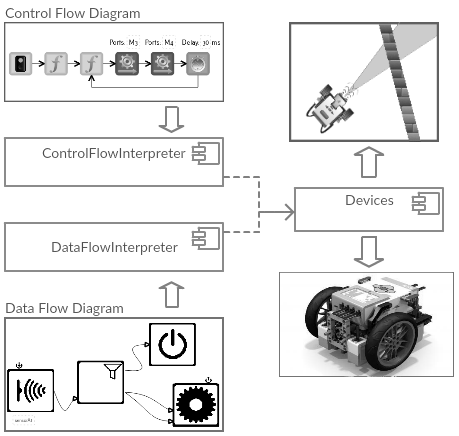
\includegraphics[width=0.9\columnwidth]{TS_Interpreter_Architecture.png}
    \caption{Diagram interpretation workflow}
    \label{image:interpretersTSArch}
\end{figure}

All interpreters, like all the rest of the environment, are written in C++/Qt. As input data they receive created diagrams in an internal representation format. There are two interpreters implemented in TRIK Studio now: one for control-flow programs and one for data-flow programs.

The interpreter of control-flow programs starts with finding the initial block of the program and then iterates according to the control flow defined by diagram arrows. Currently executed block is highlighted in the editor to show users execution status. For each block visited special factories create objects that implement the behavior of this block. In general such an object searches for a ready-to-work robot device that it needs, runs appropriate commands and passes execution to one of the blocks that the current block has an outgoing arrow to (depending on the block's semantics). Within this process no difference is made if the device is a real one or a virtual one, so the same interpretation code works for execution of a program in two out of three modes (see Section~\ref{chapter:generalDescription}).

If on any step of the interpretation a fork block is met, the interpreter launches new threads of execution, creating a new call stack for each of them. If a subprogram call block is met, its arguments are computed and put into the current call stack, and the interpretation process is repeated recursively. When processing any type of final block the interpreter removes the top frame from the call stack and the execution is being continued from the proper point of the previous diagram. If we get an empty call stack after removing the frame, the current execution thread is considered finished. This way the interpretation process is going on while the interpreter is able to find new blocks to process.

An interesting consequence of this approach is that users can change diagrams during interpretation and changes will be applied ``on the fly''. It is a convenient behavior, for example, for selecting parameters of a PID controller in a program. Meanwhile, the execution of unchanged diagram parts is optimized: block implementation objects are cached, the same is true for abstract syntax trees and type inference information for textual programs. Thus, if the program remains unchanged while being interpreted, subsequent control flow to the same parts of the diagram will employ already created objects. Diagram validation is also performed ``on the fly''. If some incorrect fragment is found, an error message is shown. It could be seen as a drawback since users get their error messages only when such errors are reached during interpretation, but this behavior is typical for all widely used interpreted textual languages.

The data-flow interpreter works in two steps. First, the interpreted diagram is being validated, implementation objects for diagram blocks are created (they are used to translate the diagram into a sequence of robot commands similar to as it was discussed for the control-flow programs interpreter). Implementation objects are connected to each other via Qt signals and slots in the same order as corresponding blocks are connected on a diagram (the Publisher-subscriber design pattern is used here). On the second step the interpreter executes each block that does not have any incoming data flows, and then each such block in its turn activates blocks that it has outgoing data flows to when the data tokens are ready. Blocks execution is performed in a pseudo-parallel way over a centralized message queue. This implementation detail distinguishes this language from all other industrial solutions (e.g. in Microsoft Robotics Developer Studio diagrams are deployed as a set of independent web services~\cite{jackson2007microsoft}). We chose this approach because this programming environment targets low-performance controllers of educational robots, that don't embrace true parallel execution of multiple programs at once. Nevertheless, the language has a process fork block that is useful while implementing complex control models mentioned above. This block is a low-level tool for execution control.

\section{Generators}
\label{chapter:generators}

One of the most interesting and demanded TRIK Studio features is generation of well-readable textual code from visual diagrams. Several languages are supported for code generation: C, JavaScript, F\#, Pascal, Russian version of C~\cite{terekhovTools} and byte code for Lego EV3 virtual machine. This section presents only code generators for control-flow programs.

As mentioned before, a visual diagram is built from blocks and arrows, defining program's \textit{control flow graph}~\cite{steven1997advanced}. All algorithmic operators like conditions, loops, switches, etc. are defined by arrows. For instance, to create an infinite loop one should create an arrow from a block to one of the previous blocks, to create \texttt{while-do} and \texttt{do-while} loops or loops with \texttt{break} statement inside it is enough to simply connect one block inside a loop with a block from the outside. It is obvious that each arrow on a diagram corresponds to a \texttt{goto} statement in the resulting code. But the code containing \texttt{goto} statements is very hard to understand, and especially is not suitable for teaching programming basics, so we decided to avoid using them in generated code as much as possible. We cannot eliminate \texttt{goto} statements completely because it is possible to create a TRIK Studio diagram that could not be expressed using standard algorithmic operators (there are algorithms for automatic translation of \texttt{goto}-containing programs into structural programs, but the result is not much better from the teaching programming point of view). On the other hand, not all modern textual programming languages support \texttt{goto} statements (for example, JavaScript does not). We call \textit{structural} diagrams that could be expressed using structural algorithmic statements (\texttt{if-then}, \texttt{if-then-else}, \texttt{while-do loop}, \texttt{do-while loop}, \texttt{while-break loop}, \texttt{switch}). Code generated from structural diagrams we also call \textit{structural}. Otherwise we say that the diagram (and the code generated from it) is \textit{not structural}. If structural code could not be generated from a given diagram, users are notified with a warning.

Considering these issues implementation of code generation subsystem in TRIK Studio required solving two non-trivial tasks, given below in a form of requirements.
 
\begin{itemize}
    \item Code generation subsystem should be organized in a way to minimize time and effort for adding of a new generator. Preferably it should be possible even for an external developer to do it.
    \item For each language (where applicable) the subsystem should support two generation modes: structural diagrams should be translated into structural code, non-structural diagrams -- into non-structural code. The success of structuring the diagram should not depend on its size and complexity.
\end{itemize}

The first task is purely of architectural nature. The solution it is shown on Fig.~\ref{image:generatorsArchitecture}. The main idea  is to divide code generation process into two steps. First, the diagram is translated into a representation independent of a target language --- a \textit{semantic tree}. Semantic trees reorder the control flow graph model into a tree model regardless of whether the diagram is structural or not. If it is, a parent node in the semantic tree always corresponds to an execution block in generated code, and its children nodes correspond to statements of this block, which exclude \texttt{goto}. An outline of the code generation process is shown in Fig.~\ref{image:generatorsArchitecture}.

\begin{figure*}[ht]
    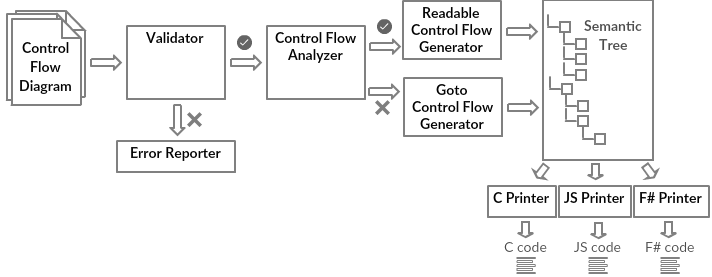
\includegraphics[width=0.6\textwidth]{TS_Generators_Architecture.png}
    \caption{Code generation subsystem's architecture}
    \label{image:generatorsArchitecture}
\end{figure*}

A code generator gets a diagram as input data. First, the diagram is traversed in a depth-first order by a validation component. Then, for each computable expression used inside block property values parsing and type inference procedure is performed. If the diagram or any code in any property value contains an error, users are notified and the code generation process terminates. If the diagram is syntactically correct, it is passed to a control flow analyzer, that is described below. Depending on if the diagram can be translated into structural code or not, an intermediate generator of code-independent diagram representation is selected, which extracts the semantic tree from the control flow graph. Finally, the semantic tree is printed into a target textual language. To achieve it, a template-based approach is used, so to create a new generator a programmer has to provide a set of such code templates and define a generator specification. For example, generation templates for condition expression in C looks like this:
\begin{verbatim}
    if (@@CONDITION@@) {
        @@THEN_BODY@@
    } else {
        @@ELSE_BODY@@
    }
\end{verbatim}

The second task is solved by a control flow analyzer module. In terms of a textual language the task is rephrased like this: by a given program containing \texttt{goto} statements create an equivalent structured program. This problem was solved by researchers in the code decompilation field~(\cite{steven1997advanced,derevenets2009structural}). For example, such an algorithm based on interval analysis of control flow graph is presented in~\cite{steven1997advanced}. With minor modifications it was implemented in TRIK Studio. It is briefly described below.

Informally speaking, an \textit{interval} is a part of a control flow graph with one input and one output. The algorithm aims to build a nesting tree for all graph intervals and is based on recursive ascend of depth-first search. On each step the algorithm tries to match a subgraph, outgoing from the current node, with each of basic interval templates (algorithmic statements that are used to structure the program). If such a template is found, the whole subgraph is folded into a single node and the process continues. The most simple example of such a template is two intervals connected with an only edge, which matches with sequential composition. If no template could be found on any step, the diagram is considered not structural. 
 
\section{Textual language parser and interpreter}
\label{chapter:parser}
TRIK Studio uses visual languages for robots programming, but arithmetic expressions, intrinsic function calls and so on are better represented with textual strings (in fact, NXT-G tries to use visual blocks even for arithmetic expressions, representing them as syntax trees, it is very inconvenient). As a textual part of a language for both visual languages TRIK Studio uses a subset of Lua 5.3 (https://www.lua.org/), customized for our needs. The decision to implement our own parser and interpreter of a textual language was made under these considerations:

\begin{itemize}
	\item we needed a small textual language with lightweight syntax and without explicit typing since it shall be used by non-programmers;
	\item we needed explicit abstract syntax tree and the ability to run type inference on it since we were going to generate code in C or EV3 bytecode, which is strongly typed;
	\item we needed to be able to customize language syntax if the need will arise;
	\item all existing implementations for such languages had interpreters without access to a syntax tree or a parser that was not reusable from C++ code;
	\item since we needed only a subset of a language (arithmetic expressions without statements, custom function and type definitions), writing custom parser was not a difficult task.
\end{itemize}

The parser and the interpreter were implemented as a separate library in QReal core, so the resulting textual language is available not only in TRIK Studio, but in all other domain-specific solutions based on QReal. Parser implementation consists of two parts --- general-purpose parser combinator library and Lua parser library implemented using parser combinators. Many projects use ANTLR (http://www.antlr.org/), boost.spirit (http://boost-spirit.com/home/), yacc (http://dinosaur.compilertools.net/yacc/) as tools for parser development, but we once again created our custom solution, mainly to avoid additional external dependencies and complication of a build process --- QReal and TRIK Studio are developed by a large community, and not everyone is happy to install additional tools and learn how to use them, especially if their work has nothing to do with syntax analysis and they are students who do not took formal languages course yet.

QReal parser combinator library supports recursive-descent parsers which are able to parse a subset of LL(1) grammars. FOLLOW($\alpha$) set is not calculated, so it limits the expressiveness of resulting grammars, but we were still able to use Lua 5.3 grammar almost as it is specified, with only minor modifications related to factorization and left recursion elimination, which shall be done anyway for LL parsers. For arithmetic expressions Precedence Climbing algorithm (see http://www.engr.mun.ca/\~theo/Misc/exp\_parsing.htm for details) was used, and it also required some minor alterations in Lua grammar. Custom modifications were made mainly on lexer level to allow, for example, to use '!=' for inequality in addition to '\verb|~=|' used in Lua. Here is a quick example of production written in C++ with our library (``statement is ';' or a list of expressions, optionally followed by '=' and other list of expressions''):
\begin{verbatim}
	// stat ::= ‘;’ | explist [‘=’ explist]
	stat = (-LuaTokenTypes::semicolon 
	    | (explist 
			   & ~(-LuaTokenTypes::equals & explist)))
\end{verbatim}

For full specification of our parser with many irrelevant technical details see https://github.com/qreal/qreal/tree/master/qrtext/src/lua. 

\verb|LuaTokenTypes::semicolon| is a token corresponding to ';', operator '-' creates a simple parser that can parse only semicolons and excludes semicolons from the AST, ``explist'' is a reference parser object, like ``stat'', defined elsewhere, '\&' combines two parsers into a parser which accepts concatenation of their corresponding strings, '|' combines two parsers into a parser that accepts alternative, '\verb|~|' creates an optional parser from its argument, which shall also be a parser. There are also operators for adding semantic actions to productions and assigning parser a name for debug purposes. When all parsers are combined in such a way, it is enough to call 'parse()' method of a resulting parser object, giving it a token stream. The parser combinator library was used for anoFther language in QReal~\cite{tikhonova2015generation}, so it is general enough to support not only Lua.

The parser returns an abstract syntax tree on which the type inference algorithm is executed, providing types for all variables and expressions. Type inference uses Hindley-Milner-style~\cite{damas1982principal} algorithm, simplified for performance reasons and extended to support overloading and coercion. Type inference is also generalised and Lua type inferer only defines inference rules for Lua-specific AST nodes, core type inference functionality is available for all QReal textual languages.

After type inference is complete, expression is ready to be evaluated by the interpreter. The interpreter allows to register intrinsic functions, also it allows to add custom variables with their values, to use current sensor values in calculations --- robot communication subsystem receives telemetry data from a robot and injects sensor readings into the interpreter, which uses them to calculate expressions.

Last notable feature of parsing/interpreting subsystem is extensive use of caching to avoid parsing or reevaluating expressions as much as possible. Program shall be interpreted in real-time, so reparsing and reevaluating expressions every several milliseconds, as required by many control algorithms, would be severe performance problem. But as mentionen before, a program can be changed by user during interpretation, values for some variables may be changed by external code, such as sensor readings changed by communication subsystem, so the interpreter keeps track of all changes and uses previously calculated values if possible.

\section{Simulator}
\label{chapter:2dModel}

2D robot simulation environment is the most stand-alone TRIK Studio subsystem. Its window is a part of TRIK Studio's user interface, but it also can be used separately. The main part of this environment is an editor for virtual world model. Using a special menu one can select one of the supported drawing tools (similar to how it is done in most graphical editors). There are two main drawing tools: drawing walls (solid objects that robots cannot move through and that are detected by robots' ultrasound and infrared sensors) and colored markers on the floor (elements that are detected by color, light sensors and virtual robots' cameras). Colored markers could be drawn in a shape of lines, cubic Bézier curves, rectangles, ellipses or any shape drawn using mouse pointer. For each marker users are able to set their its, color and fill type. 

The robot model itself is a differential two-wheeled truck. Robot model is always shown in this editor, users can place sensors onto it where they prefer. Regions where sensors scan for objects are highlighted. A separate panel shows an image of the chosen controller (Lego NXT, EV3 or TRIK), which users can interact with: clicking on an image of a button emulates controller's button click event, users can manipulate LEDs placed on controller's case or output text or images onto the controller's screen, for example,  using drawing blocks (see Section~\ref{chapter:controlFlowLanguage}).

Running the program in the simulation environment is performed in the same editor where users create their models. The world model can be changed even during program execution, putting additional walls or colored markers will take immediate effect on virtual robot's sensors. Positions and directions of the sensors themselves can also be changed in any time, which conforms with changing real robot's configuration while it is moving.

The simulation environment is built based on the Model-View-Controller design pattern. The Model contains serialized specification of the robot and the world, and it notifies all other components if any property of any object is changed. The View is subscribed to these events, all updates are immediately displayed in the editor or other simulator windows. All user actions are handled by the Controller component, which uses an intermediate command stack to be able to undo such commands on demand.

The simulation environment has two implementations of robot behavior models: ``ideal'' and ``realistic''. Within the ideal model all friction forces (for floor and walls) are ignored, and having constant motor powers the robot continues to move without any acceleration or slowdown. Any, even slightest collision with a wall will stop the robot. The realistic model takes care of thrust and friction force, when crashing into a wall the robot tries to behave like the real device. Users also have an ability to add Gaussian noise to sensor data and motor impulses. Changing between these models is done using checkboxs in the simulation settings window and could be done even during the execution of a program. 

Time in the simulation environment does not equal computer's time: there is a special centralized timeline, the speed of which can be controlled from a special panel. The same timeline is used in the diagram interpreters to match the work of timer blocks with virtual time independently of CPU's time.

\section{Automatic checking of solution correctness}
\label{chapter:constraintsChecker}

Last important subsystem described in this paper is automatic checker of constraints for TRIK Studio programs. This subsystem allows to turn a world model in a simulator to an exercise with specified success and failure conditions, which can be shared among students, and solutions (in a form of visual programs) can be automatically checked against these success conditions in the simulator, thus providing feedback without an intervention from a teacher. To create an exercise one needs to specify two things:

\begin{itemize}
    \item what parts of a simulated world are fixed and can not be changed by a student (walls and figures on a floor, robot starting position, sensors and their orientations and so on);
    \item program on a special constraints definition language which specifies success and failure conditions for a solution.
\end{itemize}

Constraints are described in a special XML-based definition language. A program in this language is a set of events $\{ e_1, e_2, ..., e_n \}$, where each event $e_i$ is a triple $(id_i, c_i, T_i)$:

\begin{itemize}
    \item $id_i$ --- event id: an internal label by which other parts of a program may refer to this event, can be empty;
    \item $c_i$ --- condition, under which the event is raised, a formula in a first-order predicate calculus without quantification;
    \item $T_i$ --- ordered list of triggers $[ t_{i_1}, t_{i_2}, ..., t_{i_n} ]$. Each trigger specifies an action that shall be done when event condition $c_i$ becomes true.
\end{itemize}

Each event is specified by its XML node in a program. An event can be specified in a \textit{canonical} form, or in a form of a \textit{constraint}. The event in a canonical form is a triple $(id_i, c_i, T_i)$. The event in a constraint form is a triple $(id_j, c_j, message_j)$. A constraint is interpreted as an event $(id_i, $$\neg$$c_i, [ fail(message_j) ])$, where $fail(message_j)$ is a trigger that stops simulation and reports a $message_j$ error message. In other words, a constraint is the event that is raised when given condition is violated and reports this violation to a user. Events in a form of constraints are added to a language for pragmatical reasons only, because it is much more convenient to specify conditions like ``robot $x$ shall not leave area $a$'' or ``robot $x$ shall have a set of sensors $s$ connected'' as constraints instead of events. Time limits are a special case of such constraints. A time limit shall be specified for each constraint definition program so the constraints checker will not run the simulation indefinite amount of time if all constraints are satisfied but success event is never triggered. The checker verifies that a time limit is set before execution of a program, and if not, considers it as a semantic error.

Let us briefly describe predicates, function symbols and elementary triggers used in the language. Predicate symbols are divided into these groups.
\begin{itemize}
    \item Comparison predicates $>$, $<$, $\leq$, $\geq$, $=$, $\neq$.
    \item Spatial predicates. They have an ``item $x$ is located inside area $y$'' form.
    \item Event state predicates $settedUp(id_i)$ and $dropped(id_i)$, denoting active and inactive events accordingly. Active events can be raised when their corresponding condition is satisfied, events in inactive state will not be raised (and their triggers will not be executed) even when condition is satisfied.
    \item Time predicate $timer(t)$, which is initially false, becomes true after $t$ ticks of model time and stays true afterwards.
    \item Other ``syntactic sugar''.
\end{itemize}

Function symbols are the following.
\begin{itemize}
    \item Constants of different types (integer, floating-point, string, colour, geometrical and so on).
    \item $variableValue(id)$ symbol that denotes a value of a variable with identifier $id$. Variables are internal to the constraints checking program (i.e. do not represent simulation state) and can be useful for implementing complex conditions like counting the times that robot does some action.
    \item Arithmetical and geometrical operations over other values: for example, an absolute value of a number or a distance between two points.
    \item Comparison of forms of two figures using Levenshtein distance. It is useful to compare images drawn on robot display to an ideal image specified in an exercise.
    \item $objectState(path)$ symbol allows to get state of a simulated robot devices or objects of a simulated world. $path$ argument shall contain a path to a desired property in a hierarchy of objects in world model. Such path will be translated into a sequence of C++ object property references using Qt Reflection mechanism, so this symbol provides a bridge between constraints definition and the simulator environment.
\end{itemize}

Finally, elementary triggers are the following:
\begin{itemize}
    \item $success$, $fail(message)$ control the checker's state. First trigger reports exercise as successfully checked, second reports error and marks simulation result as a failure;
    \item triggers that set variable values and change properties of a simulated world or a robot device (complementary to $objectState$ function), they allow, for example, to set random number generator seed to make possible testing solutions that use random number generator;
    \item triggers that control event state: every state can activate or deactivate every other state (including itself), it allows to specify rather complex checking scenarios, like visiting waypoints in a correct order within given amount of time.
\end{itemize}

An example of a simple program in the constraints description language is given in Listing~\ref{code:constraints}.

\captionsetup[figure]{name=Listing}
\setcounter{figure}{0}

\begin{figure*}[!t]
\begin{verbatim}
<!-- Root element, contains all constraints -->
<constraints>

    <!-- Mandatory time limit constraint -->
    <timelimit value="2000"/>

    <!-- Constraint on robot location -->
    <constraint failMessage="Robot left the allowed area!">
        <inside objectId="robot1" regionId="myspace"/>
    </constraint>

    <!-- Success criteria for a program: robot must say "Hello" using speech synthesis 
		     and draw a smile on a screen -->
    <event settedUpInitially="true">
        <conditions glue="and">
            <equals>
                <objectState object="robot1.shell.lastPhrase"/>
                <string value="Hello"/>
            </equals>
            <equals>
                <objectState object="robot1.display.smiles"/>
                <bool value="true"/>
            </equals>
        </conditions>
        <trigger>
            <success/>
        </trigger>
    </event>

</constraints>
\end{verbatim}
\caption{Example of constraints specification in TRIK Studio simulator model}
\label{code:constraints}
\end{figure*}

Architecturally the constraints checking system is a standalone module which uses TRIK Studio core and the simulator model as shared libraries. The simulator model and robotic kit support in TRIK Studio are frequently extended with new devices, options and features, so Qt Reflection mechanism is used to access objects and their properties from constraint specifications. It allows to extend the TRIK Studio core without modifications in the constraints checking system itself, new properties immediately become available from the constraints description language. The constraints checker subscribes to events from the simulation model as another view (in MVC pattern sense) and checks constraints on every tick of model time. It may seem ineffective, but only active constraints are checked each timer tick (and only a few constraints are active at any given time), so constraints checking almost does not affect the performance.

The described language has proven to be quite effective at specifying spatial and temporal constraints on a system state. It is more expressive than, for example, temporal logic or topological temporal logic languages which are used for specification of formal constraints on robot behavior in recent works~(\cite{mordvinov2016formal,kress2007s,bugaichenko2007development,dmitriev2013adaptation}). The constraints checking system is also used for functional testing of TRIK Studio on continuous integration server. For more information on this (and other details of TRIK Studio testing) see in~\cite{mordvinov2016testing}.

This functionality is also used as an automatic checker of exercises for MOOC on Stepik platform. Without such checker it would be impossible to provide feedback to possibly large number of students, making course much less interactive. From a technical point of view the checker is a set of scripts which launch ``headless'' interpreter (i.e. interpreter without GUI) on a correct field with correct constraints. Checker is hooked up into the Stepik infrastructure and runs in a separate Docker container when a new solution is submitted. The checker has several fields and corresponding constraint descriptions for each task (from one to five), each solution is checked against all those fields to test that it works in different situations and is not hardcoded. Fields are hidden from users, but error reporter output does gets displayed, so students can guess what went wrong (in our opinion it is better than traditional ACM ICPC system, where only a number of incorrect test and a general type of error are reported).

The checker can also send a visual representation of a field with a trace of a robot to a client. A trace consists of points of a robot trajectory and values reported by its sensors, and this trace can be played back by a web application described in~\cite{zakharov2016web}. This web application also allows to actually create solutions for almost all tasks from the course right in the browser, form a correct TRIK Studio save file and run it on a server on the checker, playing back the result, so a student perceives this as ``TRIK Studio in a browser''. This application works standalone, but is not integrated into the Stepik course yet due to technical difficulties related to the Stepik infrastructure.

\section*{Conclusion}
\label{chapter:conclusion}

Technical description of the TRIK Studio robots programming system was presented. TRIK Studio now has about ten thousand users across the globe, according to Google Analytics data. Now it supports English, Russian and French languages. It is open source (https://github.com/qreal/qreal) and has large and active community developing it. TRIK Studio has about 100K lines of code (excluding QReal core, which also has size of about 120K LOC), written in C++ with Qt. Good reception of TRIK Studio in educational robotics community may be viewed as a proof that modeling environment created with domain-specific platform (QReal in this case) can actually compete with visual programming environments written specifically for robots programming.

Future work consists of two major development vectors: improvements of the existing system and new research projects based on it. Improvement tasks are gathered from teachers, pupils and students which use TRIK Studio, and there is already several hundreds of such tasks tracked. For example, support for new robotic platforms (such as Arduino, STM32), simulator improvements (more precise physics simulation, multiagent systems simulation and so on), support for more textual languages (like Python, Pascal). Research projects that are currently using TRIK Studio as a technical base include research in domain-specific visual languages field and formal methods field of study. For example, we are creating technology to automatically generate visual domain-specific language using metainformation from packages of robotic middleware (ROS~\cite{quigley2009ros} is currently considered), that visual language will be able to link middleware nodes together thus configuring environment for a particular robot. Research in formal methods aims to formalize semantics of used visual languages to be able to apply formal verification and synthesis methods to diagrams.

\bibliographystyle{IEEEtran}
\bibliography{trikStudioEnglish}

\end{document}